\documentclass{article}
\usepackage{spconf,amsmath,amssymb,graphicx,booktabs,url,microtype,array}
\usepackage[T1]{fontenc}
\setlength{\emergencystretch}{2em}

\title{CONTACT OR CONTOUR? SUPERVISING A BOUNDARY MATTERS MORE THAN WHICH BOUNDARY FOR SEPARATING TOUCHING NUCLEI}
\name{Varun Kumar Dasoju$^{1}$, Qingsu Cheng$^{2}$, Zeyun Yu$^{1}$}
\address{University of Wisconsin--Milwaukee, Milwaukee, WI, USA\\
$^{1}$Department of Computer Science; $^{2}$Department of Biomedical Engineering\\
\texttt{vdasoju@uwm.edu, chengq@uwm.edu, yuz@uwm.edu}}

\begin{document}
\maketitle

\begin{abstract}
Supervising the borders where nuclei touch, as in the winning 2018 Data Science Bowl solution, is a popular way to keep touching nuclei from merging, but its effect is rarely separated from the design choices that change with it. We measure it in matched ten-seed experiments with image-paired confidence intervals on BBBC039, two NucleusSegData test sets (Huh7, HepG2), and 53 external DSB2018 images, against full-contour, semantic-watershed, and scratch-trained Cellpose baselines. Adding a boundary head, with marker-based decoding, to the watershed baseline raised aggregated Jaccard index (AJI) by 0.027--0.041 on BBBC039 and 0.035--0.036 externally, and object F1, the pre-specified endpoint, by 0.023--0.028 and 0.028--0.040. Which boundary was supervised mattered less: on BBBC039 a contact-only target beat the full-contour target by 0.014 AJI (46 of 50 images), robust to seed and image resampling and to test-time augmentation, with fewer merged touching nuclei (21\% vs.\ 27\%), but by only 0.005 in object F1. Elsewhere the contact advantage was small or conditional: externally the targets tied in AJI and contact gained 0.011 object F1; Huh7 excluded a gain of the BBBC039 size; HepG2 gained only after re-tuned post-processing; and a contact head lowered Cellpose's AJI. Scratch-trained Cellpose, which has no boundary head, had the best panoptic quality on every test set. For foreground-based networks, supervising a boundary is worth doing; which boundary is a secondary choice to confirm on held-out data.
\end{abstract}
\begin{keywords}
nucleus instance segmentation, touching nuclei, boundary supervision, Cellpose, empirical comparison
\end{keywords}

\section{Introduction}
Nuclear instance masks support cell counting, morphometry, and spatial analysis. A segmentation that covers two touching nuclei with one object barely changes foreground Dice yet corrupts counts and per-cell measurements; on BBBC039, 29\% of nuclei touch another. Instance methods separate nuclei with contour classes~\cite{chen2016dcan,caicedo2019evaluation}, distance or shape representations~\cite{naylor2019segmentation,schmidt2018stardist,graham2019hovernet}, gradient flows~\cite{stringer2021cellpose}, or multi-stage attention~\cite{gunesli2020attentionboost}. A simpler, widely used heuristic is to supervise where nuclei touch: U-Net up-weighted the gaps between touching cells~\cite{ronneberger2015unet}, a multiclass loss added a touching-region class~\cite{guerreropena2018multiclass}, and the winning 2018 Data Science Bowl solution predicted touching borders together with masks~\cite{topcoders2018dsb,caicedo2019nucleus}.

New methods typically change backbone, decoder, targets, and training recipe together, and single-run comparisons can mistake seed variance for method effects~\cite{bouthillier2021variance}. We ask how much contact targets help relative to the choices that change with them, separating matched from composite contrasts. Our contributions are:
(1)~a ranking of design effects (Fig.~\ref{fig:effects}): where both were measured, adding a boundary head raised AJI by 0.027--0.041 and object F1 by 0.023--0.040, while the boundary target changed AJI by at most 0.014 on any of four test sets, and not consistently;
(2)~a multi-seed, image-paired test of contact versus full-contour targets with identical network, loss, selection, and decoder, robust in AJI to seed and image resampling on BBBC039; and
(3)~an error analysis of where contact targets help (fewer merged touching nuclei on BBBC039) and where they do not (Huh7, inside Cellpose).

\begin{figure*}[t]
\centering
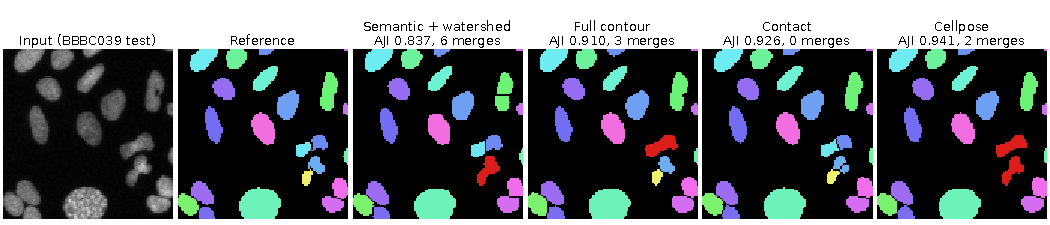
\includegraphics[width=\textwidth]{fig_contact_examples.pdf}
\caption{BBBC039 test crop chosen by a fixed rule (contact model's upper-median seed by object F1, its median image, the window with most contacts; same seed for all models). Objects take the colour of the reference nucleus they mostly cover; red: merging objects; grey: unmatched. Titles: whole-image AJI, merging objects.}
\label{fig:examples}
\end{figure*}

\section{Methods}
\textbf{Boundary targets.} Let $L$ be the reference instance map (0: background), $N_k(x)$ the $k$-neighbourhood of pixel $x$, and $\mathcal D$ dilation by a radius-1 disk. The two targets differ only in whether the neighbour that defines a boundary may be background:
\begin{equation}
\begin{split}
C&=\{x:L(x)>0,\ \exists x'\!\in\!N_8(x):L(x')\notin\{0,L(x)\}\},\\
B&=\{x:L(x)>0,\ \exists x'\!\in\!N_4(x):L(x')\neq L(x)\},
\end{split}
\end{equation}
with contact target $c=\mathcal D(C)\cap\{L>0\}$ and full-contour target $b=\mathcal D(B)\cap\{L>0\}$~\cite{chen2016dcan,caicedo2019evaluation}. Thus $c$ keeps only borders between nuclei, the cue that decides separation, whereas $b$ also marks nucleus--background edges that the foreground head already resolves; on BBBC039, $c$ covers 0.34\% of pixels and $b$ 4.9\%. Targets are built at native resolution and resized (nearest neighbour) with the image; the foreground target $y_f=\{L>0\}$ is left intact.

\textbf{Network and loss.} A UNet++~\cite{zhou2018unetpp} with an ImageNet-pretrained EfficientNet-B7 encoder~\cite{tan2019efficientnet} (decoder widths 256--16) ends in one two-channel layer whose sigmoids give foreground $p_f$ and boundary $p_c$, trained on $c$ or, for the control, on $b$. The loss is
\begin{equation}
\begin{split}
\mathcal L={}&\tfrac12[\mathcal L_D(p_f,y_f)+\mathcal L_B(p_f,y_f)]\\
&+\tfrac14[\mathcal L_D(p_c,c)+\mathcal L_{B,w}(p_c,c)],
\end{split}
\end{equation}
with soft Dice $\mathcal L_D$ and binary cross-entropy $\mathcal L_B$; $\mathcal L_{B,w}$ weights positive pixels by $w=\min(50,\max(1,(1-r)/r))$ for batch target ratio $r$, which sits at the cap for $c$ and near 20 for $b$, so the target contrast includes this weighting difference.

\textbf{Decoding.} A boundary prediction may split a foreground component but never joins or deletes one: (i)~$F=\{p_f>.5\}$ after filling holes and removing objects smaller than $s$ pixels ($s=16$; NucleusSegData: chosen on training images); (ii)~markers are the 4-connected components of $F\setminus\{p_c>\tau\}$ with at least $s$ pixels, $\tau\in\{.3,\dots,.7\}$ chosen on validation; (iii)~within each 4-connected component of $F$, every pixel takes its Euclidean-nearest marker in that component (component-preserving), or the component is flooded from its markers by watershed on $p_c$; (iv)~a component without markers stays one object. Given the foreground, separation errors therefore arise only from missed boundaries (merges) or spurious ones (splits). An earlier global nearest-marker decoder, found faulty after test scoring, handed marker-less components to neighbours and more than doubled the contact--contour AJI gap (.870 vs.\ .838); no reported result uses it.

\textbf{Matched controls and baselines.} With identical network, loss, selection, and decoder, we compare $c$ with $b$ and with a \emph{carved} target that, like one variant of the 2018 winning solution, removes contact pixels from $y_f$ (decoded with $F=\{p_f>.5\}\cup\{p_c>\tau\}$). A one-channel \emph{semantic} network is decoded by connected components (CC) or distance-transform watershed ($h$-maxima on a smoothed distance map, $h,\sigma$ chosen on validation); its checkpoints are selected by validation object F1 after watershed, as for the two-head models. Cellpose~\cite{stringer2021cellpose} (v3.1.1) is trained from scratch on the same split (its released models saw Data Science Bowl images, which share BBBC039's source) with its default recipe (500 epochs; inference diameter: median square-root nucleus area, 25/32 pixels; Cellpose's convention, 28/36, changed AJI by $\le$0.004); flow and probability thresholds are chosen on validation. We add contact supervision to it as a fourth output trained with the contact loss above (decoded normally or by splitting objects along predicted contacts), and as weights $1+Wc$ on Cellpose's flow and probability losses, screened on validation ($W\in\{3,10\}$) by a pre-set rule (object F1 $+0.002$, no seed declining).

\textbf{Error taxonomy.} A reference nucleus is \emph{merged} if its majority lies in a predicted object that also holds another nucleus's majority, \emph{split} if it holds the majority of two or more objects, and \emph{unmatched} without an IoU$>$0.5 match; strata (touching another nucleus; small, $<$128 native pixels) were fixed before analysis. Rates pool nuclei per seed, then average over seeds.

\section{Experimental setup}
\textbf{Data.} BBBC039v1 has 200 $520\!\times\!696$ Hoechst images of U2OS cells~\cite{ljosa2012annotated,caicedo2019nucleus}; we use the official 100/50/50 split. Expanded NucleusSegData~\cite{gunesli2020attentionboost,koyuncu2018object} has 25 training, 11 Huh7, and 25 HepG2 test images. For zero-shot testing we use the 53 grey-scale fluorescence images of the 2018 Data Science Bowl stage-1 test set~\cite{caicedo2019nucleus}, none duplicating a BBBC039 image (template-matching correlation $\le$0.58).

\textbf{Protocol.} Base models resize percentile-normalized images to $512^2$ and train for 20 epochs (AdamW, learning rate $3\times10^{-4}$, cosine decay, flips and rotations); checkpoints and $\tau$ are chosen on the 50 validation images by object F1 before test scoring. Base two-head rows re-decode these locked choices with the component-preserving decoder; TTA rows reselect decoder and $\tau$ on validation from one grid shared by both targets; all re-decodings are reported. A final setting trains at native resolution (random $512^2$ crops, 40 epochs) and averages eight dihedral test-time augmentations (TTA); a validation-only search (six recipes, two seeds) then chose 200 epochs with intensity jitter. NucleusSegData has no validation set: models train for 60 epochs (Cellpose: 500), keep the final epoch, and choose post-processing on training images.

\textbf{Endpoints and statistics.} Foreground Dice (DICE1), AJI~\cite{kumar2017aji}, panoptic quality (PQ)~\cite{kirillov2019panoptic}, and object F1 over IoU 0.50:0.05:0.90~\cite{caicedo2019evaluation}, as image means; NucleusSegData uses the Bilkent nucleus F1~\cite{koyuncu2018object} (one-to-one matches covering half of each other, pooled per subset). The locked protocols designated object F1 as primary; AJI, a main endpoint of prior BBBC039 work~\cite{wang2022aswnet,yi2022segmentgraph}, was emphasized after the locked runs and is reported alongside it. Contact vs.\ contour (base protocol, decoder corrected after test scoring) is the confirmatory contrast; all other intervals, including boundary-head effects, are exploratory and unadjusted. Count error is the mean absolute per-image count difference. Seeds are averaged within each test image; 95\% percentile CIs use 10,000 image-paired bootstrap resamples, conditional on the trained models; a two-way bootstrap that also resamples each arm's seeds checks retraining variability.

\section{Results}
\begin{table}[t]
\centering\footnotesize
\caption{BBBC039 official test set, mean (seed SD) over ten seeds unless marked ($^\S$five seeds). Two-head rows use the component-preserving decoder (final setting: it or watershed on $p_c$, chosen on validation); $^\P$200 epochs, intensity jitter, chosen on validation. Literature: published values, same split; $^\ddagger$scored on expanded-interior targets.}
\label{tab:bbbc}
\setlength{\tabcolsep}{2.1pt}
\resizebox{\columnwidth}{!}{\begin{tabular}{@{}lrrrr@{}}\toprule
Model & DICE1 & AJI & PQ & Obj.-F1\\\midrule
\multicolumn{5}{@{}l}{\emph{Foreground-based, base protocol ($512^2$)}}\\
Semantic + CC & .9653(.0013) & .6779(.0133) & .7406(.0080) & .7520(.0084)\\
Semantic + watershed & .9653(.0013) & .8303(.0050) & .8371(.0029) & .8583(.0031)\\
Full-contour target & .9637(.0016) & .8568(.0042) & .8541(.0044) & .8817(.0044)\\
Carved foreground & .9650(.0025) & .8692(.0036) & .8619(.0039) & .8865(.0033)\\
Contact target & .9660(.0023) & .8712(.0057) & .8610(.0047) & .8865(.0040)\\\midrule
\multicolumn{5}{@{}l}{\emph{Final setting (TTA, validation-selected decoder)}}\\
Full contour, $512^2$ & .9676(.0006) & .8682(.0033) & .8664(.0025) & .8934(.0027)\\
Contact, $512^2$ & .9692(.0010) & .8792(.0051) & .8713(.0029) & .8959(.0030)\\
Contact, native resolution & .9715(.0008) & .8895(.0040) & .8807(.0028) & .9049(.0023)\\
+ searched recipe$^\P$ & \textbf{.9721}(.0003) & .8965(.0023) & .8835(.0016) & .9069(.0013)\\
\midrule
\multicolumn{5}{@{}l}{\emph{Flow-based (Cellpose 3, from scratch)}}\\
Cellpose & .9702(.0016) & \textbf{.9053}(.0035) & \textbf{.8884}(.0036) & .9119(.0031)\\
+ contact head$^\S$ & .9700(.0004) & .8975(.0013) & .8872(.0009) & \textbf{.9121}(.0011)\\
\midrule
ASW-Net$^\ddagger$~\cite{wang2022aswnet} & .9645 & .9020 & .8665 & --\\
BISSG~\cite{yi2022segmentgraph} & .9482 & .8680 & .8629 & --\\
Caicedo U-Net~\cite{caicedo2019evaluation} & -- & -- & -- & .8980\\\bottomrule
\end{tabular}}
\end{table}

\begin{figure}[t]
\centering
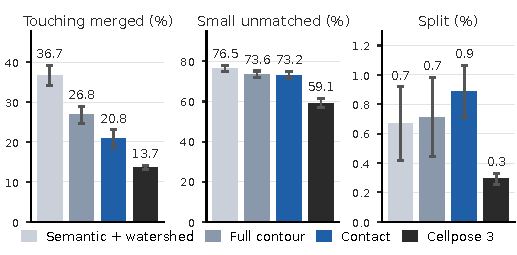
\includegraphics[width=\columnwidth]{fig_error_profile.pdf}
\caption{Error profile on BBBC039 test (base protocol; mean and seed SD over ten seeds) as a percentage of the 1,650 touching, 509 small ($<$128 pixels), and 5,720 reference nuclei.}
\label{fig:errors}
\end{figure}

\begin{figure}[t]
\centering
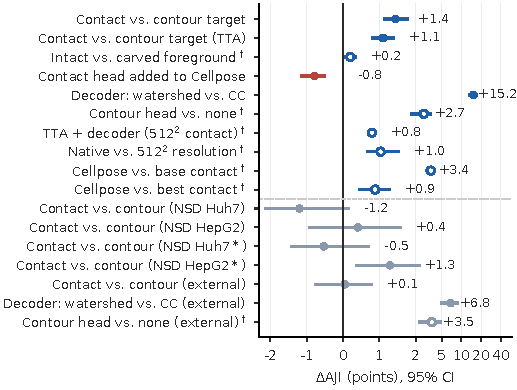
\includegraphics[width=\columnwidth]{fig_effects.pdf}
\caption{Effect of each design choice on AJI (points, AJI$\times$100; mean of image-paired differences, 95\% bootstrap CI; symmetric-log axis). Rows above the dashed line use BBBC039 test; below it, NucleusSegData (NSD; $^\ast$widened grid and TTA for both targets) and the external DSB2018 images. Open markers ($\dagger$): composite comparisons that also change decoder, reconstruction, recipe, or resolution.}
\label{fig:effects}
\end{figure}

\subsection{Supervising a boundary mattered more than which one}
Supervising contacts instead of contours added $0.014$ AJI ($[.011,.018]$; 46/50 images) and object F1 $+0.005$ ($[.002,.008]$); with TTA (same decoders and selection for both), $0.011$ ($[.008,.014]$; 45/50; object F1 $+0.003$, $[-.0001,.005]$). Resampling seeds as well as images kept both AJI intervals above zero ($[.009,.020]$, $[.006,.016]$), but not the object F1 interval with TTA ($[-.001,.006]$; base $[.0002,.010]$). Adding a boundary head$^\dagger$ to the watershed baseline mattered more (exploratory; the decoder changes with it): AJI rose by $0.041$ ($[.032,.051]$; 48/50) with contact and $0.027$ ($[.019,.035]$) with contour, $0.012$ ($[.004,.021]$) more than the target effect, and object F1 by $0.028$ ($[.022,.035]$) and $0.023$ ($[.017,.030]$), $0.019$ ($[.012,.026]$) more. On identical semantic predictions, a tuned watershed instead of connected components (a no-separation floor) raised AJI by $0.152$ ($[.126,.178]$). Correcting the faulty decoder moved AJI by $0.018$ for contour networks ($[.015,.022]$; 49/50) but $0.001$ for contact networks. Carving contacts out of the foreground changed AJI by $0.002$ ($[.0004,.0036]$), and a validation-searched recipe raised it by $0.007$ ($[.004,.010]$). Cellpose exceeded our best contact model by $0.009$ ($[.004,.013]$; seed and image resampling $[.004,.014]$).

\subsection{On BBBC039, contact targets merged fewer nuclei}
Contact supervision was accompanied by (Fig.~\ref{fig:errors}) fewer merges of touching nuclei, from 36.7\% (watershed) and 26.8\% (full contour) to 20.8\% (contact minus contour $-5.9$ points, $[-7.7,-4.4]$, seed and image resampling $[-8.6,-3.5]$; 44/50 images), and of all nuclei, from 10.8\% and 8.2\% to 6.3\%, while splits stayed below 1\% (0.67\%, 0.71\%, 0.89\%), although splits of touching nuclei rose from 1.3\% (contour) to 2.3\%. All three models undercounted, and the per-image count error fell from 10.1 (watershed) and 7.2 (contour) to 6.6 nuclei. Unmatched small nuclei, by contrast, were similar across foreground-based models (73--77\%); training at native resolution lowered this to 64\% for the contact model (no TTA), so resizing explains only part of it.

\subsection{A contact head did not help Cellpose}
Cellpose merged 13.7\% of touching nuclei, split 0.29\% of all nuclei, and left fewer small nuclei unmatched (59\%; Fig.~\ref{fig:errors}). In the tested recipe, the auxiliary contact head (five seeds) lowered AJI relative to the ten baseline seeds by 0.008 ($[.005,.012]$; worse on 39/50 images) without materially changing PQ or object F1 ($-0.001$, $+0.000$)(equal seeds, resampled: $-0.007$, $[-.011,-.002]$); validation never selected contact-based splitting in any seed. The contact-weighted loss failed its validation screen and was not tested.

\subsection{Second benchmark and external images}
\begin{table}[t]
\centering\footnotesize
\caption{Expanded NucleusSegData, Bilkent nucleus F1; ours: mean (seed SD) over ten seeds, component-preserving decoder; AttentionBoost: five published runs~\cite{gunesli2020attentionboost}. $^\ast$Widened training-selected grid and TTA. $^\S$Five seeds.}
\label{tab:nucleusseg}
\setlength{\tabcolsep}{3pt}
\begin{tabular}{@{}lrr@{}}\toprule
Method & Huh7 & HepG2\\\midrule
Multi-task~\cite{gunesli2020attentionboost} & .934(.009) & .869(.005)\\
AttentionBoost~\cite{gunesli2020attentionboost} & .954(.005) & .919(.008)\\
Full contour & .9541(.0062) & .9162(.0079)\\
Contact & .9533(.0057) & .9170(.0080)\\
Full contour$^\ast$ & .9609(.0039) & .9240(.0029)\\
Contact$^\ast$ & .9575(.0051) & .9286(.0069)\\
Cellpose 3, scratch$^\S$ & \textbf{.9715}(.0038) & \textbf{.9426}(.0038)\\\bottomrule
\end{tabular}
\end{table}
On expanded NucleusSegData (Table~\ref{tab:nucleusseg}), the contact model matched the published multi-stage AttentionBoost in nucleus F1 and was higher with a widened training-selected post-processing grid and TTA. In the base setting the targets did not differ detectably (Huh7 AJI $-0.012$, $[-.024,.002]$, 2/11 images; HepG2 $+0.004$, $[-.009,.016]$), with nucleus F1 differences below 0.001; the Huh7 interval excludes the BBBC039 gain of 0.014. Re-decoding both targets with the widened grid and TTA (Table~\ref{tab:nucleusseg}, $^\ast$) kept Huh7's direction ($-0.005$, $[-.015,.007]$) but favoured contact on HepG2 ($+0.013$, $[.004,.023]$; 16/25; nucleus F1 $+0.005$). Scratch-trained Cellpose reached .971 and .943, 1.1 and 1.4 points above the best foreground-based model, and the best PQ (.870 and .795 vs.\ at most .859 and .785). \begin{table}[t]
\centering\footnotesize
\caption{Zero-shot results on 53 external DSB2018 fluorescence images (BBBC039-trained base models, ten seeds; count error in nuclei per image).}
\label{tab:external}
\setlength{\tabcolsep}{3pt}
\begin{tabular}{@{}lrrrrr@{}}\toprule
Model & DICE1 & AJI & PQ & Obj.-F1 & Count err.\\\midrule
Semantic + watershed & .803 & .585 & .555 & .493 & 12.2\\
Full-contour target & \textbf{.812} & .620 & .581 & .521 & \textbf{9.1}\\
Contact target & .811 & .621 & .589 & .532 & 9.3\\
Cellpose & .796 & \textbf{.633} & \textbf{.633} & \textbf{.584} & 13.7\\\bottomrule
\end{tabular}
\end{table}
Applied unchanged to the 53 external images (Table~\ref{tab:external}), a boundary head again improved on the semantic watershed in AJI (contour $+0.035$, $[.022,.049]$; contact $+0.036$) and object F1 ($+0.028$, $+0.040$). The targets tied in AJI ($+0.001$, $[-.008,.008]$) and PQ ($+0.008$, $[-.0001,.016]$); contact had higher object F1 ($+0.011$, $[.002,.021]$; 35/53) but merged more touching nuclei (30.9\% vs.\ 27.6\%; $+3.3$ points, $[1.3,4.8]$), a difference not robust to seed resampling ($[-0.4,7.3]$). Cellpose exceeded the contact model in PQ ($+0.044$, $[.016,.072]$) but not detectably in AJI ($+0.012$, $[-.016,.039]$); its count error was larger by 4.4 nuclei per image ($[2.4,6.9]$), yet it left far fewer predicted objects unmatched (pooled 12\% vs.\ 24\%), so the foreground models' smaller count error partly reflected unmatched predictions offsetting missed nuclei.

\section{Discussion and conclusion}
Where both were measured, supervising a boundary helped more than the choice of boundary, in AJI and in the pre-specified object F1. Contact beat contour robustly in AJI on BBBC039, on HepG2 only after re-tuned post-processing, and externally only in object F1; it did not help on Huh7 or inside Cellpose. Cellpose, without a boundary head, was the strongest pipeline (best PQ on every test set), so boundary supervision is a lever for foreground-based networks, not a requirement. In practice: add a boundary head, tune the decoder (never reassign marker-less components), compare with a flow-based model, and confirm the target choice on held-out data. Limitations: fluorescence images only, one annotation each; the targets differ in effective positive weight; the decoder fix followed test scoring; the native-resolution and searched settings lack a contour arm; one Cellpose recipe; no StarDist~\cite{schmidt2018stardist} or foundation-model baselines~\cite{archit2025microsam,pachitariu2025cellposesam}.

\section{Compliance with ethical standards}
This research study was conducted retrospectively using open-access images of cultured cell lines (BBBC039~\cite{ljosa2012annotated}, NucleusSegData~\cite{gunesli2020attentionboost}, DSB2018~\cite{caicedo2019nucleus}). It involved no human subjects or animals, and ethical approval was not required.

\section{Acknowledgments}
This work was supported by U.S. Department of Energy grant DE-SC0025403. The authors declare no competing interests. OpenAI Codex and Anthropic Claude assisted with analysis scripts, statistics, figures, and language editing of all sections; the authors designed and verified the experiments and take responsibility for the manuscript. Code and per-image results: \url{https://github.com/vkd14/contact-or-contour}.

\let\oldbibitem\bibitem\renewcommand{\bibitem}{\setlength{\itemsep}{0.6pt}\oldbibitem}
\bibliographystyle{IEEEbib}
{\small\bibliography{references}}
\end{document}
